
%%%%%%%%%%%%%%%%%%%% file CSMC_MUME_LaTeX_Template.tex %%%%%%%%%%%%%%%%%%%%%
%
% This is the LaTeX source for the instructions to authors using
% the LaTeX document class 'llncs.cls' for contributions to
% the Journal of Creative Music Systems.
% Copyright: http://www.springer.com/lncs       Springer Heidelberg 2006/05/04
%
% It may be used as a template for your own input - copy it
% to a new file with a new name and use it as the basis
% for your article.
%
% NB: the document class 'llncs' has its own and detailed documentation, see
% ftp://ftp.springer.de/data/pubftp/pub/tex/latex/llncs/latex2e/llncsdoc.pdf
%
%%%%%%%%%%%%%%%%%%%%%%%%%%%%%%%%%%%%%%%%%%%%%%%%%%%%%%%%%%%%%%%%%%%

\documentclass[runningheads,a4paper]{llncs}


\usepackage{amssymb}
\usepackage{amsmath}
\setcounter{tocdepth}{3}
\usepackage{graphicx}
\usepackage{caption}
\usepackage{subcaption}
\captionsetup{labelfont=bf, labelsep=period,compatibility=false}
\usepackage{apacite}
\newcommand{\keywords}[1]{\par\addvspace\baselineskip
\noindent\keywordname\enspace\ignorespaces#1}

\renewcommand{\baselinestretch}{0.96}
\raggedbottom
\pagestyle{headings}

\begin{document}


\mainmatter  % start of an individual contribution

% first the title is needed
\title{A Study on Neural Models for Target-Based Computer-Assisted Musical Orchestration}

% a short form should be given in case it is too long for the running head
\titlerunning{Neural Models for Target-Based Computer-Assisted Musical Orchestration}

% the name(s) of the author(s) follow(s) next
%
% NB: Chinese authors should write their first names(s) in front of
% their surnames. This ensures that the names appear correctly in
% the running heads and the author index.
%
\author{Carmine Emanuele Cella\inst{1}\and Luke Dzwonczyk\inst{1}\and Alejandro Saldarriaga-Fuertes\inst{1}\and Hongfu Liu\inst{1}\and H\'el\`ene-Camille Crayencour\inst{2}}
%
% if the names of the authors are too long for the running head, please use the format: AuthorA et al.
\authorrunning{Carmine Emanuele Cella et al.}
\titlerunning{{\em 2020 Joint Conference on AI Music Creativity}, Full Paper}


% the affiliations are given next; don't give your e-mail address
% unless you accept that it will be published
\institute{CNMAT - University of California, Berkeley \and Centrale Sup\'elec, L2S, Univ. Paris-Saclay, CNRS \\ \email{carmine.cella@berkeley.edu, dz.luke@berkeley.edu }}

%
% NB: a more complex sample for affiliations and the mapping to the
% corresponding authors can be found in the file "llncs.dem"
% (search for the string "\mainmatter" where a contribution starts).
% "llncs.dem" accompanies the document class "llncs.cls".
%

\maketitle

\begin{abstract}
In this paper we will perform a preliminary exploration on how neural networks can be used for the task of target-based computer-assisted musical orchestration. We will show how it is possible to model this  musical problem as a classification task and we will propose two deep learning models. We will show, first, how they perform as classifiers for musical instrument recognition by comparing them with specific baselines. We will then show how they perform, both qualitatively and quantitatively, in the task of computer-assisted orchestration by comparing them with state-of-the-art systems. Finally, we will highlight benefits and problems of neural approaches for assisted orchestration and we will propose possible future steps.

\keywords{computer-assisted orchestration, CNN, LSTM, ResNet, Orchidea}

\end{abstract}

%
\section{Introduction}\label{sec:introduction}

The development of computational tools to assist and inspire the musical composition process constitutes an important research area known as \emph{Computer-Assisted Composition (CAC)} \cite{FerVic2013, Ari2005}. Within CAC, target-based computer-assisted orchestration is a compelling case of how machine learning can be used for {enhancing} and {assisting} music creativity \cite{Maresz2003}. 

Target-based computer-assisted orchestration takes a target sound as an input and attempts to find instrumental samples that best match the target given a specific similarity metric and a set of constraints. A solution to this problem is a set of orchestral scores that represent the mixtures of audio samples in the database, ranked by similarity with the target sound. 



\begin{figure}
	\centering
	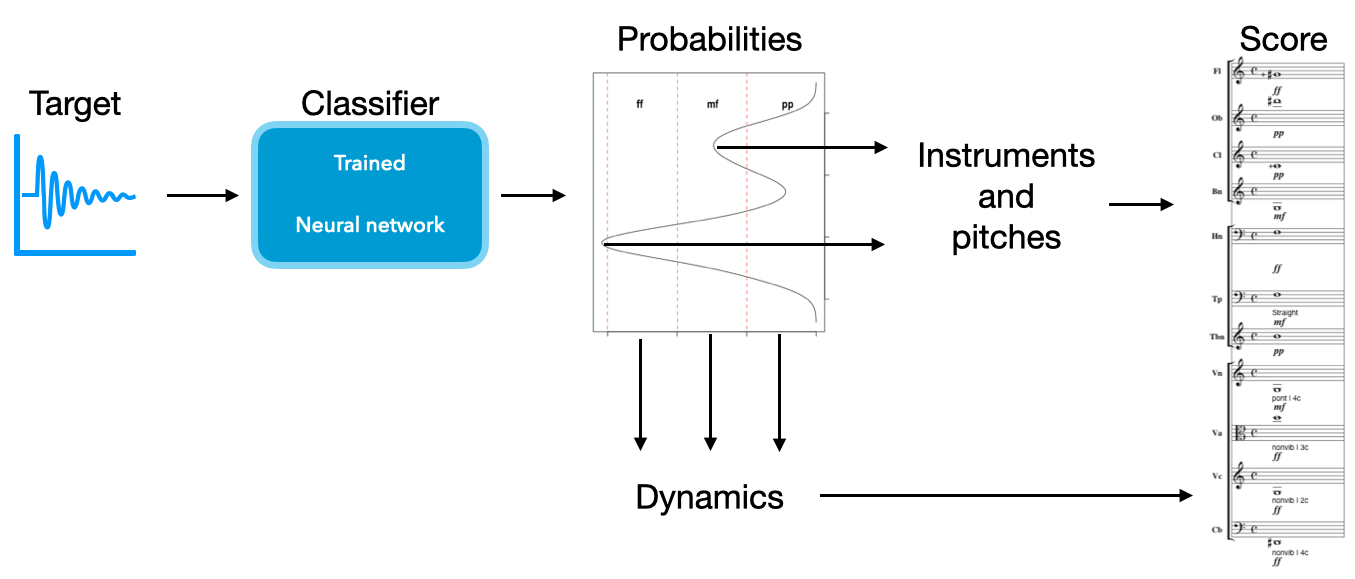
\includegraphics[scale=0.20]{../latex/figs/method.png}
	\caption{An overview of the proposed method for assisted orchestration with neural models. Instruments and pitches are determined as peaks of the output probability distribution, while the dynamics are computed by quantizing the probabilities. \label{fig:method}}
\end{figure}

The approach studied in \cite{Carpentier2010} consists in finding a good orchestration for any given sound by searching combinations of sounds from a database with a multi-objective optimization heuristics and a constraint solver that are jointly optimized. Both the target sound and the sounds in the database are embedded in a feature space defined by a fixed feature function and each generated combination of sounds is evaluated by using a specific metric. This method has been substantially improved in \cite{Cella18, Cella2020} and is implemented in the \emph{Orchidea} toolbox for assisted orchestration (\url{www.orch-idea.org}), currently considered the state-of-the-art system for assisted orchestration.

In this paper, we try a different approach to this problem by experimenting with deep neural architectures. The main idea is to train a model to classify combinations of real instruments and then use it for orchestration. A typical solution for assisted orchestration is a set of triples \emph{instrument-pitch-dynamics} such as \{\texttt{Flute C6 pp, Bassoon C4 mf, Bassoon G4 ff}\}. By training a neural network with real combinations of instrumental notes, it will acquire the ability to identify the presence of each instrument and its associated pitch by building the appropriate latent representation. Thus, when an unknown target sound is given as input, the network will identify which are the best instruments to match the target sound, and it will be able to  deconstruct a complex mixture of timbres into individual instrument notes. This method is motivated by the good results obtained in previous research on musical instruments identification \cite{Benetos07, Kitahara05} and the more recent use of deep neural networks for musical classification \cite{lostanlen16, Bian19}. 

In this paper we perform preliminary experiments with two deep architectures: a convolutional neural network (CNN) with a long short-term memory (LSTM) unit and \emph{ResNet}, a well known residual architecture that already yielded good results for image classification \cite{He15}. We chose to use a CNN because of its success in audio classification \cite{Hershey17} and we decided to include an LSTM unit in it because of its ability to learn long term dependencies in data \cite{Hochreiter97}, which is important given the temporal nature of audio. The codebase for this paper can be found at: \url{https://github.com/dzluke/DeepOrchestration}.
\\

\section{Neural models}
\label{sec:models}


%\begin{figure}
%	\centering
%	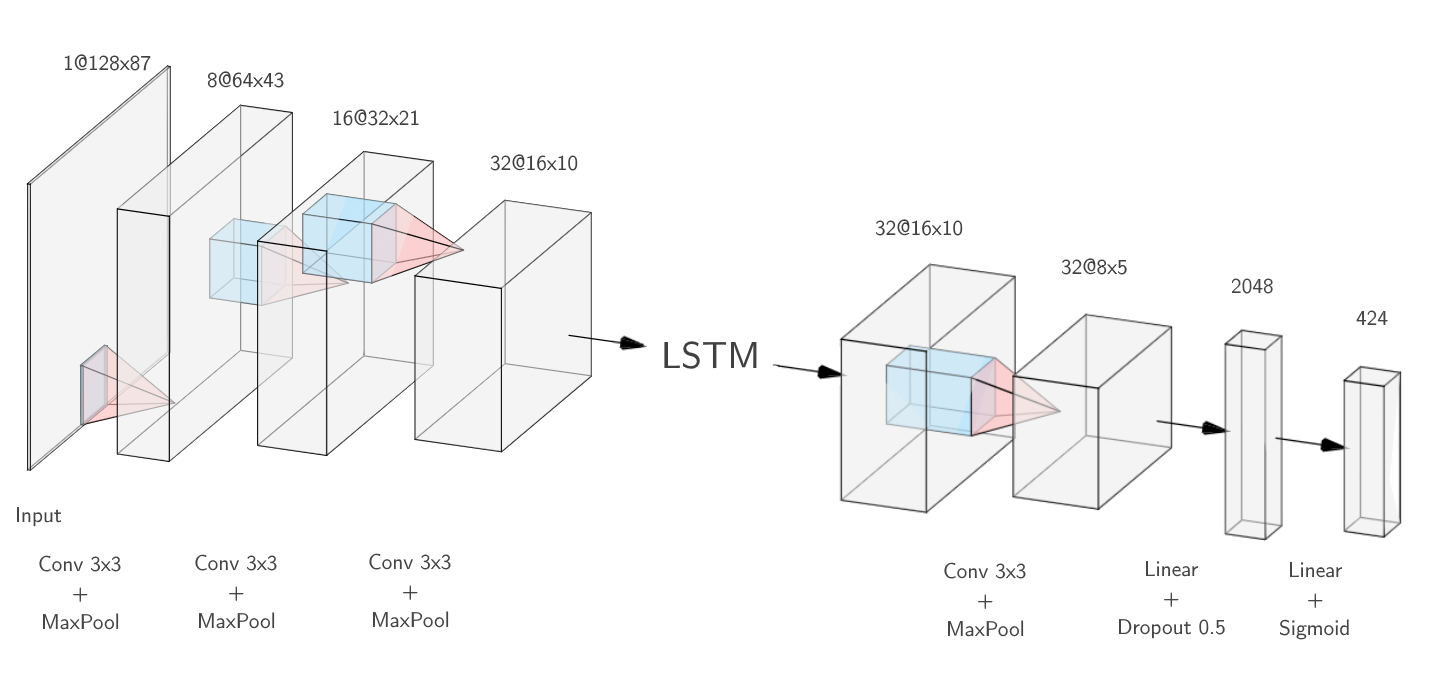
\includegraphics[scale=0.22]{../latex/figs/CNN_LSTM_diagram.png}
%	\caption{Diagram of the CNN with LSTM architecture. \label{cnn_lstm}}
%\end{figure}

\subsection{From Orchestration to Classification}

In this paper, we model assisted orchestration as a classification problem. The general methodology is as follows:
\begin{enumerate}
\item we train specific models to classify the instruments present in combinations of sounds from a database of instrument notes, up to ten simultaneous instruments;
\item we then pick the best classifier and we feed into it an unknown sound to be classified;
\item since the output of the classifier will be in the form of the probability that specific instruments are present in the sound, we use this information to synthesize an orchestration for the target sound;
\item finally, we evaluate the generated orchestration against state-of-the-art systems for computer-assisted orchestrations.
\end{enumerate}

In other words, the classifiers learn how to take a complex combination of pitches and timbres and deconstruct it into its original parts.

A complete orchestration solution, however, would normally be made by triples of \textit{instrument-pitch-dynamics}. It is difficult to frame this problem as classification, since we would need to have a very high number of classes. Moreover, for the nature of the samples we use (a typical sample is in the form \texttt{Flute-C4-pp}, as described in \ref{sec:dataset}), each class would be represented by a single sample. For this reasons, our models were not trained to determine \textit{instrument-pitch-dynamics} triples but instead \textit{instrument-pitch} pairs.


\subsection{Dataset}
\label{sec:dataset}

To create the input data for training the classifiers, we used the \emph{TinySOL} database. TinySOL is a subset of the Studio On Line (SOL) database created by IRCAM \cite{Cella2020b}. TinySOL contains 1,529 samples from 12 instruments. The instruments come from different orchestral families: strings, woodwinds, and brass. Each sample is one instrument playing a single note in the \emph{ordinario} playing style, with one of three dynamics: \textit{pp}, \textit{mf}, or \textit{ff} (for example \texttt{Flute-C4-pp} or \texttt{Clarinet-D5-mf}). 

%The instruments and ranges over which they were recorded are summarized in table \ref{tab:ranges}. 

For a given number of instruments $N$, each input to our model is a combination of $N$ TinySOL samples chosen among an orchestra of 10 instruments. The data is generated by selecting $N$ random TinySOL samples, leading to a variety of instruments, pitches, and dynamics; we did not allow the same instrument to be chosen more than three times in order to ensure variety in the mixtures. Then the chosen samples are combined to be played simultaneously and normalized by the number of instruments. The resulting combination has a sample rate of $44100$Hz and is padded or trimmed to be exactly 4 seconds long. The Mel spectrogram of the mixture is computed using an FFT hop length of 2048 samples (the window of each FFT is $46$ms wide) and 128 Mel bins. Therefore, the Mel features fed to the model are matrices of size $128\times 345$.

The choice of using the Mel spectrogram as input features for classification models is common in music information retrieval \cite{McKinney2003} and can be considered to be an appropriate representation of sound and musical signals. %The Mel spectrogram is generated using an FFT hop length of 2048 samples (the window of each FFT was $46$ms wide), and a number of Mel bins equal to 128. Therefore, the Mel features fed to the model were matrices of size $128\times 345$. We used the Librosa package in Python to compute the features; more details on the exact computations can be found in \cite{mcfee15}. %The choice of the hop length was made by doing a compromise between the amount of information extracted by each FFT window, and the ability to capture changes in the dynamic, assuming that no change faster than $10$ms would be allowed.
Such setup proved to be successful in \cite{Salamon17}.


\subsection{Data Augmentation}

In order to increase variability in the generated data for the neural models, we also used two methods of data augmentation as described in \cite{Salamon17, Bhardwaj17}; more specifically, we used pitch shifting and partial feature dropout.

Pitch shifting was applied on the TinySOL samples each time they were selected to generate a new combination. We performed a small pitch shift by reading the samples with different sample rates: a small difference in sample rate will slightly modify the duration and the perceived pitch if played at the normal sample rate. In practice, the sample rates used for this data augmentation were within $5\%$ of the actual $44100$Hz.

Partial feature dropout was performed on the feature matrix itself of input samples, the Mel spectrogram. We chose random columns and rows of the matrix to zero out. %For a given matrix, each column and each row had individually a $1\%$ chance to be set to 0, which yielded an average of $1.28$  columns and $3.45$ rows being zero-ed out. 
This method of data augmentation aimed to be more resilient to the possible variations in the recording of the instruments.

\subsection{Baselines}
\label{sec:baseline}

In order to get a better sense on the complexity of the problem, we tested three baseline classifiers: support vector machine (SVM), random forest (RF), and K-nearest neighbours (KNN). We used the implementations provided in the \emph{scikit-learn }library for Python \cite{scikit-learn}. 
In this case, differently from the neural models, the features used are the MFCCs of the resulting combination; as the number of features is more manageable for parametric classifiers. We found SVM to have the highest accuracy of the three classifiers across all experiments.

We started with a simplification of our problem. We performed experiments in which two instruments were selected, and the classifier attempted to identify instrument and pitch \emph{class} of the samples. For two instruments, SVM had an accuracy of 39.9\% and RF had an accuracy of 17.5\%. As the number of instruments used in combination increased, the accuracy dropped sharply. With three instruments, SVM accuracy was 11.1\%, with four instruments it was 2.7\%. Clearly, these classifiers were not going to be able to achieve meaningful results with the full setting of our problem.

%\begin{table}
%  \centering
%  \caption{Comparison of accuracies between SVM and RF. Each data point is a combination of two TinySOL samples, where at least one of the samples is from one of the two instruments specified for that experiment. For the samples drawn from one of the two instruments, the pitch class of that sample is identified. For a sample not from one of the two instruments, the classifier simply attempted to identify that a sample from one of the non-specified instruments was present. In this setting, there are 25 classes: 24 from the 12 pitch classes from 2 instruments, and 1 class that specified whether an instrument that is not one of the two specified is present. \label{tab:baselines}}
%    \begin{tabular}{|c|c|c|c|} 
%    	  \hline
%      \textbf{Instr. 1} & \textbf{Instr. 2} & \textbf{SVM Acc.} & \textbf{RF Acc.}\\
%      \hline
%      Violin & Flute & 38.8\% & 9.8\% \\
%      \hline
%      Violin & Trumpet & 33.8\% & 9.1\% \\
%      \hline
%      Violin & Cello & 34.8\% & 6.3\% \\
%      \hline
%      Cello & Viola & 32.1\% & 5.8\% \\
%      \hline
%      Oboe & French Horn & \textbf{39.9\%} & \textbf{17.5\%} \\
%      \hline
%    \end{tabular}
%\end{table}

%In the rest of this section, we will show the classification results of the two neural models. 

\subsection{CNN with LSTM}

The first deep model we trained as a classifier for musical instruments and pitches was a CNN with a LSTM unit, whose structure is inspired by the success in \cite{Salamon17}. The LSTM unit was added in order to provide a way to learn long term dependencies in the data \cite{Hochreiter97}, which is relevant given the sequential nature of audio.

%CNNs show good performance on classification problems for their ability to extract spatial features, and have shown success in audio classification \cite{Hershey17}. LSTM units provide a way to learn long term dependencies in the data \cite{Hochreiter97}, which is relevant given the sequential nature of audio.

Our architecture is made of four convolutional layers and two fully connected layers. Each convolutional layer is followed by a BatchNorm layer, a ReLU activation layer and a $2 \times 2$  MaxPool layer with a stride of 2. The kernel size is $3 \times 3$ with a stride of 1 and a padding of 1. The number of filters are 8, 16, 32, and 32.

Following the first three convolutional layers, there is an LSTM layer which outputs 32 matrices. After the LSTM layer, there is a final convolutional layer yielding a tensor of dimensions $32\times 8 \times 21$. We flatten the outputs and feed them into a fully connected layer with Dropout, then another another fully connected layer. Finally, the sigmoid function is applied to the final layer. Since each class is independent, we are able to take the sigmoid activation and use binary classification for each class. %The model architecture is shown in Figure \ref{cnn_lstm}.

\subsection{ResNet}

The second and deeper model that we trained as classifier was the well known deep residual network \emph{ResNet} \cite{He15}. Specifically, we used 18-layer ResNet, which allows information to pass directly from the input to the final layer of each block. To make the model more suitable to our problem, we decided to use an architecture with 4 blocks whose outputs are of size 32, 64, 32 and 32 respectively.

\subsection{Classification Results}

During training, the loss function used to optimize the inner parameters of the model was binary cross entropy, as it is the common choice for multiclass multilabel classification frameworks. However, the value of the loss function alone is difficult to interpret.


\begin{figure}
  \center{
  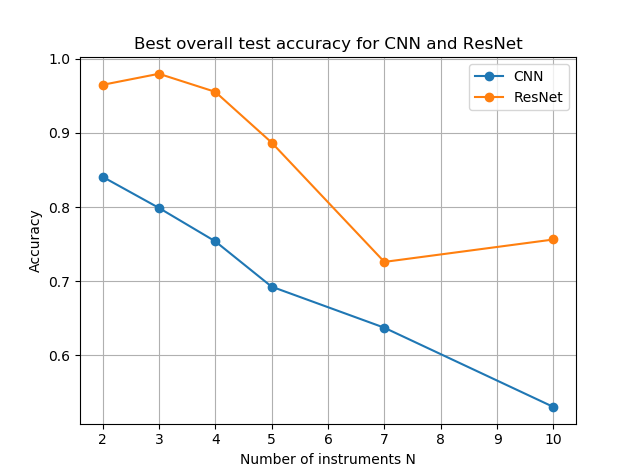
\includegraphics[scale=0.4]{../latex/figs/CNN_vs_ResNet.png}}
  \caption{Best overall accuracy for CNN with LSTM (50 epochs, 200k samples per epoch) and ResNet (20 epochs, 400k samples per epoch) depending on the number of instruments in the combinations used for training. \label{cnn_vs_resnet}}
  \end{figure}
  
%For this reason we created a complementary function $f$ to be used for evaluation only. This function compares a vector of expected outputs $\overline{X}$ with the estimated output from the model $\hat{X}$ by using the following function
%
%\begin{equation}
%f(\overline{X}, \hat{X}) = \frac{1}{N}<\overline{X}, M_N(\hat{X})>
%\label{eval}
%\end{equation}
%\begin{equation}
%M_N(\hat{X})_i = \left\{\begin{array}{ll}
%1 \text{ if } i \in I_N(\hat{X})\\
%0 \text{ otherwise}
%\end{array}\right.
%\label{NMax}
%\end{equation}
%and $I_N(\hat{X})$ is the set of indices containing the $N$ first maximums of the vector $\hat{X}$. More specifically, the function $M_N(\hat{X})$ takes as an input a vector of probabilities and outputs a vector where only the positions of the $N$ first maxima are set to 1. This new vector would be the orchestration of $N$ instruments given by the model. Thus, the function $f$ simply outputs the proportion of the estimated orchestration that matches the expected one.
For this reason, the evaluation was done by comparing the proportion of estimated orchestration samples, chosen among the samples that output the highest probability, that matched the expected orchestration.

Different experiments were made by varying the number $N$ of samples in each mixture. We used an orchestra of 10 instruments: French Horn, Oboe, Violin, Viola, Cello, Flute, Trombone, Bassoon, Trumpet in C and Clarinet in Bb. Then, for both CNN with LSTM and ResNet, we computed the maximum accuracy over the epochs. 
%The CNN was trained on 200,000 generated samples over 50 epochs, and ResNet was 	trained on 400,000 generated samples over 20 epochs. Fig. \ref{cnn_vs_resnet} shows the best overall test accuracy achieved by both models across the number of samples $N$.
ResNet outperforms the CNN regardless of the number of samples used in the combination. This result is consistent with previous research \cite{He15}, as residual networks usually perform well in classification problems.


\begin{figure}
  \centering
  \begin{subfigure}{.52\textwidth}
    \centering
    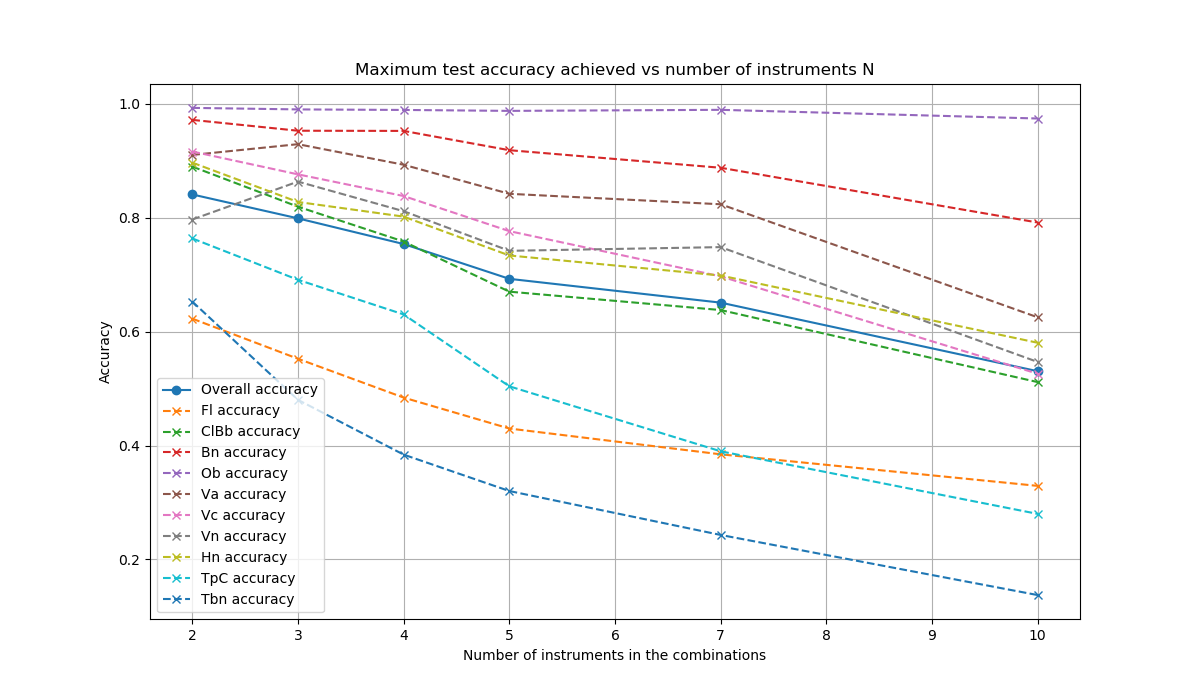
\includegraphics[width=0.9\linewidth]{../latex/figs/Acc_vs_N_CNN.png}
    \caption{CNN with LSTM}
    \label{best_acc_cnn}
  \end{subfigure}%
  \begin{subfigure}{.52\textwidth}
    \centering
    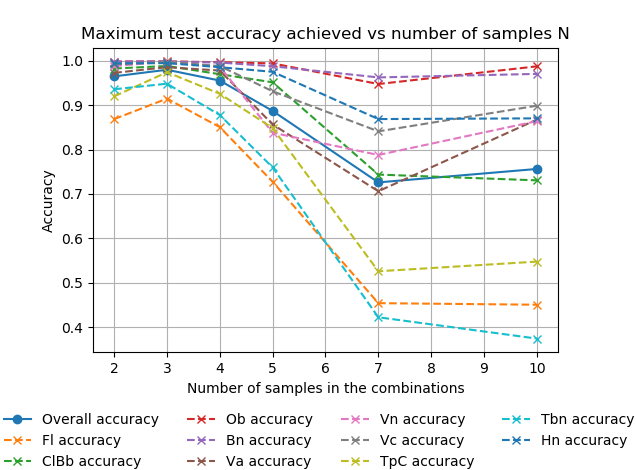
\includegraphics[width=0.9\linewidth]{../latex/figs/Acc_vs_N_ResNet.png}
    \caption{ResNet}
    \label{best_acc_resnet}
  \end{subfigure}
  \caption{Best overall accuracy and for each instrument obtained by the CNN with LSTM and the ResNet depending on the number of instruments in the combinations}
  \end{figure}

  
Fig. \ref{best_acc_cnn} and Fig. \ref{best_acc_resnet} show the maximum test accuracy for each model. For ResNet, the variance in accuracy is much smaller until $N$ reaches 5, at which point it becomes similar to the CNN. The results on both figures show consistency on the relative accuracy of instruments, which was for us the first step towards the validation of this method. Flute, Trombone and Trumpet yield the worst results for both models. 

While it is not easy to explain these differences in accuracy, we hypothesize this being related to the nature of peculiar spectral and temporal morphology of each instrument. For example, flute notes tend to exhibit a steep spectral rolloff, with most of the energy captured by the first few partials. Moreover, the noisy nature of the transient portions of these notes is not well represented by frequency-based descriptions such as Mel spectra. These two factors combined, could make the disentanglement of the flute from the analyzed combination more difficult.

Strings give similar results across both models. An interesting point to notice is the very high accuracy of Oboe on both models. This could indicate that there is an optimal spectral shape that maximizes the probability of being detected in such classification framework.


\section{Orchestration Experiments}
\label{sec:orchestration}

After training the neural models for classification, we finally tested them for the task of target-based computer-assisted orchestration. 

To orchestrate, a target sound is input to the model, and the 10 classes with the highest probability are extracted. These 10 classes are the instrument-pitch pairs that are most represented in the target, and can be from any combination of the 10 instruments. 

Since we decided not to train our models to classify the dynamics of a sample, the dynamics are determined by the probability of each sample as output by the model. If the model outputs a probability higher than $0.66$ for a sample, the fortissimo version of the sample is used. A probability between $0.33$ and $0.66$, is mezzoforte and less than $0.33$ is pianissimo. The idea behind this quantization is that samples that are the most represented in the target should appear as the loudest in the orchestrated solution.

In order to test our models for orchestration, we used 15 targets from the Orchidea distribution. These targets represent a variety of signal types but are mostly static, in the sense that they do not change sensibly over time. Some of the targets were made of instrumental samples and chords, others are bells or gongs, and some do not feature any musical instruments

\begin{table*}
	\centering    
  \resizebox{\columnwidth}{!}{\begin{tabular}{|c|c|c|c|c|c|c|c|c|c}
     \hline
      \textbf{Model} & \textbf{Ob + Bn} & \textbf{Bn} & \textbf{Bass cl.} & \textbf{Bell 1} & \textbf{Bell 2} & \textbf{Multiph. 1} & \textbf{Car horn} & \textbf{Boat} $\ldots$ \\
      \hline
      CNN with LSTM & 0.17 & 0.28 & 0.70 & 0.55 & 0.26 & \textbf{1.10} & 0.68 & \textbf{1.12} $\ldots$  \\
      \hline
      ResNet & 0.34 & 0.50 & 0.48 & 0.59 & 0.45 & 0.90 & 0.49 & \textbf{1.16} $\ldots$ \\
      \hline
      \hline
      \textbf{$\ldots$} & \textbf{Wind harp} & \textbf{Chord 1} & \textbf{Multiph. 2} & \textbf{Chord 2} & \textbf{Gong} & \textbf{Scream} & \textbf{Brass} & \textbf{Average}  \\
      \hline
      $\ldots$ & 0.55 & 0.79 & 0.70 & 0.57 & 0.73 & \textbf{1.14} & 0.79 & 0.71\\
      \hline
      $\ldots$  & 0.61 & 0.86 & 0.51 & 0.37 & 0.71 & \textbf{1.03} & \textbf{1.05} & 0.66 \\
      \hline
    \end{tabular}}
    \caption{Quantitative comparison of orchestrations as ratios to Orchidea. Eqn. \ref{distance} was used to compute distances between orchestrations and targets. What is shown is the ratio between the distance of Orchidea's solution to the target and our solution's distance to the same target. A value less than 1 means that our model performed worse (i.e. had a larger distance), and a value greater than 1 means our model performed better than Orchidea. The last column shows the ratio of the average distances for the model across all targets.}\label{orch_eval}
\end{table*}

\subsection{Evaluation}

We evaluated our orchestrations both qualitatively and quantitatively by comparing our solutions to the solutions generated by Orchidea, the state-of-the-art system for computer-assisted orchestration. 
In order to have a fairer comparison, we did not allow Orchidea to use any of its advanced features: we did not apply any symbolic constraints or harmonic analysis and we forced it to use all 10 instruments in each solution.

%Orchidea implements many advanced features that are not supported by our models. For example, it is able to apply symbolic constraints to the search, hence allowing only specific instrumental combinations or playing styles. It is also able to reduce the search space by applying harmonic analysis on the target sound, and create sparse solutions that do not use every instrument specified.
%This creates a fairer comparison, since our models are unable to create constrained or sparse solutions.

Qualitative evaluation was done through an acoustic inspection of the solution, paying close attention to timbre and pitch. For targets that had harmonic content, it was noted if the partials present in the target were also represented in the orchestrated solution.

For quantitative evaluation, we used the distance metric defined in Eqn. \ref{distance} to calculate differences in timbre between targets and solutions. This metric is proposed in \cite{Cella2020} as part of the cost function used in Orchidea during the optimization. The equation takes in the full FFT of the target $x$ and full FFT of the solution $\tilde{x}$. Then for each bin $k$ of the FFT, it calculates the absolute difference between the values. The differing values of $\lambda_1$ and $\lambda_2$ allow the metric to penalize the solution in different ways.

\begin{equation}\label{distance}
d(x, \tilde{x}) =\lambda_1 \sum_k \delta_{k1}(x_k - \tilde{x}_k) + \lambda_2 \sum_k \delta_{k2}|x_k - \tilde{x	}_k| \\
\end{equation}
where $\delta_{k1} = 1 \text{  if  } x_k \ge \tilde{x}_k, 0 \text{  otherwise}$; and $\delta_{k2} = 1 \text{  if  } x_k < \tilde{x}_k, 0 \text{  otherwise}$.

A comparison of distances between our solutions and targets and Orchidea's solutions and targets is in Table \ref{orch_eval}. While our model is not able to outperform Orchidea, it shows consistent results. We find that the CNN and ResNet give similar accuracies during training, but perform differently when tasked with orchestrating targets. Overall, CNN seems to better emulate the timbre in its orchestrations, where ResNet is better for recreating the harmonic content of the target. You can listen to the targets and orchestrated solutions from Orchidea, ResNet, and the CNN with LSTM at \url{https://dzluke.github.io/DeepOrchestration/}.


\section{Conclusions}
\label{sec:conclusions}

Target-based computer-assisted orchestration through deep learning models seems a promising path, thanks to the ability of deep networks to classify individual instruments and pitches out of dense combinations of samples. This work, however, represents only a preliminary study of the potential of these methods for the task of assisted orchestration. 

The first natural extension would be to support sparsity in our models. Our current models orchestrate all targets using a constant number of instruments and are not able to drop specific instruments from the solution. This does not take into account the density of different targets. Sparse solutions, in which the model decides how many samples should be used to best represent the target, would allow a small number of samples to be used for sonically sparse sounds and many to be used for sonically dense sounds. %This would generate more meaningful orchestrations that would compare more favourably to the state of the art.

Another important extension would be to create a more powerful embedding spaces for the target and combinations. In \cite{Gillick19} the authors propose to use LSTM-based models to predict the embedding features for the combinations used during the optimisation process in assisted orchestration. We believe that by combining their prediction model with our classification models we could generate more faithful representations and improve the overall quality of generated orchestrations.


%\subsection{Interpreting the Latent Space}
%
%After training the CNN with LSTM for $N=10$ samples per combination, it is possible to visualize the filters applied to the input layer after layer. Figs. \ref{latent0}-\ref{latent5} show the successive outputs of each layer of the convolutional network. \carmine{I put here all the intermediary features of the CNN with LSTM. I don't find any particular conclusion other than saying that LSTM seems to focus more on vertical components rather than horizontal, ie time over frequency}
%
%\begin{figure}
%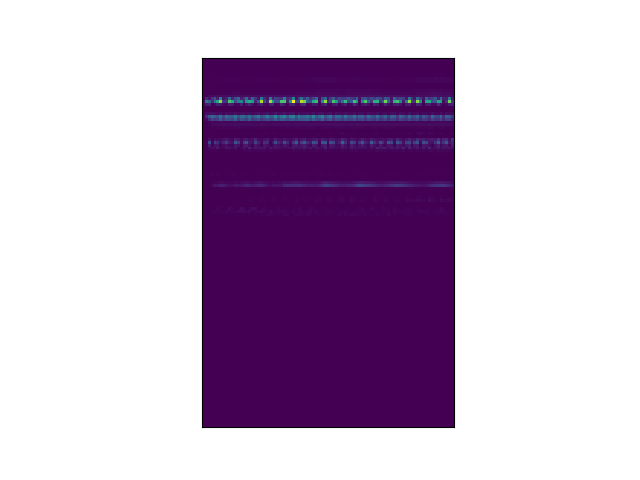
\includegraphics[scale=0.5]{figs/latent_space_layer0.png}
%\caption{Initial feature matrix used as input of the model \label{latent0}}
%\end{figure}
%
%\begin{figure}
%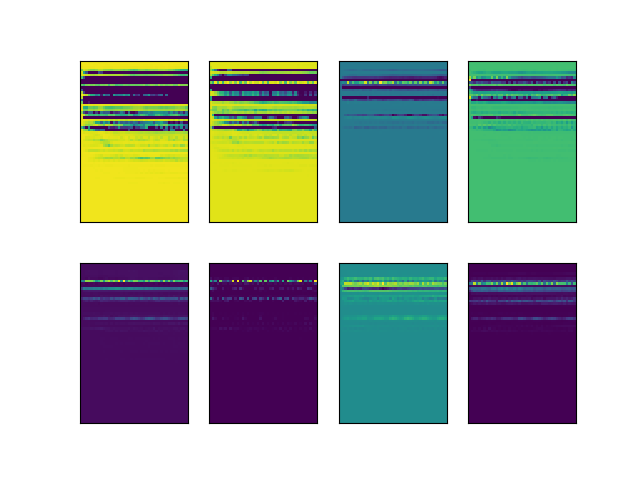
\includegraphics[scale=0.5]{figs/latent_space_layer1.png}
%\caption{Intermediary features after the first convolutional layer of the CNN with LSTM. \label{latent1}}
%\end{figure}
%
%\begin{figure}
%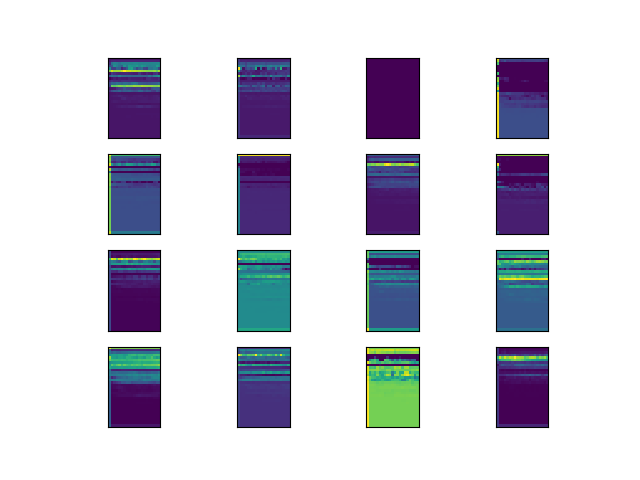
\includegraphics[scale=0.5]{figs/latent_space_layer2.png}
%\caption{Intermediary features after the second convolutional layer of the CNN with LSTM. \label{latent2}}
%\end{figure}
%
%\begin{figure}
%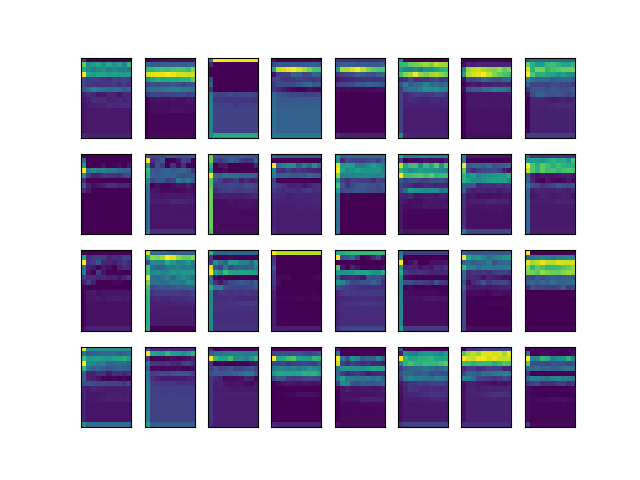
\includegraphics[scale=0.5]{figs/latent_space_layer3.png}
%\caption{Intermediary features after the third convolutional layer of the CNN with LSTM. \label{latent3}}
%\end{figure}
%
%\begin{figure}
%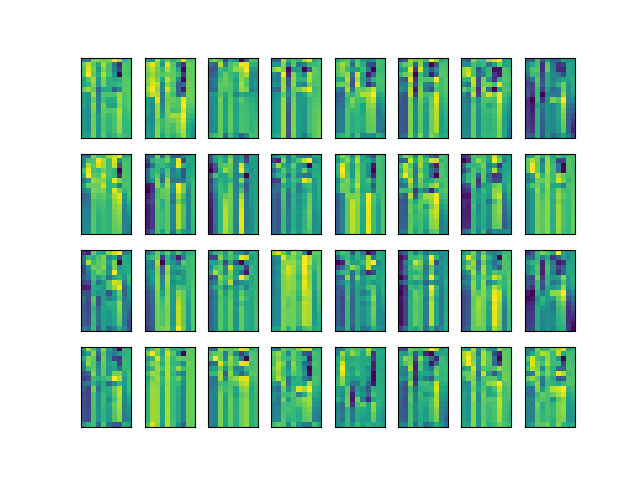
\includegraphics[scale=0.5]{figs/latent_space_layer4.png}
%\caption{Intermediary features after the LSTM layer. \label{latent4}}
%\end{figure}
%
%\begin{figure}
%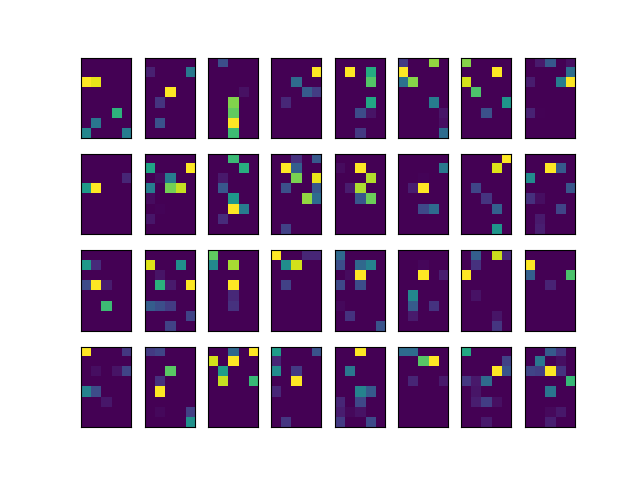
\includegraphics[scale=0.5]{figs/latent_space_layer5.png}
%\caption{Intermediary features after final convolutional layer of the CNN with LSTM. \label{latent5}}
%\end{figure}


\bibliographystyle{apacite}
\bibliography{paper}

\end{document}

